\documentclass[sigconf]{acmart}

\usepackage{hyperref}

%\usepackage{endfloat}
%\renewcommand{\efloatseparator}{\mbox{}} % no new page between figures

\usepackage{booktabs} % For formal tables

\settopmatter{printacmref=false} % Removes citation information below abstract
\renewcommand\footnotetextcopyrightpermission[1]{} % removes footnote with conference information in first column
\pagestyle{plain} % removes running headers


\begin{document}
\title{Big Health Data from Wearable Electronic Sensors (WES) and 
the Treatment of Opioid Addiction}

\author{Sean M. Shiverick}
\affiliation{%
  \institution{Indiana University Bloomington}
}
\email{smshiver@indiana.edu}

%%%%%%%%%%%%%%%%%%%%%%%%%%%%%%%%%%%%%%%%%%%%%%%%%%%%%%%%%%%%%%%%%%%%%%%%%%%%%%%%%%

\begin{abstract}
Wearable electronic sensors (WES) and mobile health applications can be used to
collect vital health data to supplement traditional forms of treatment for opioid
addiction and may be used to predict risk factors related to overdose death. 
\end{abstract}

\keywords{Health Informatics, Wearable Sensors, Addiction Treatment, i535, HID335}

\maketitle

%%%%%%%%%%%%%%%%%%%%%%%%%%%%%%%%%%%%%%%%%%%%%%%%%%%%%%%%%%%%%%%%%%%%%%%%%%%%%%%%%%

\section{Introduction}

In the increasingly connected digital age, personal electronic devices are 
generating huge volumes of data with important applications for health 
informatics. Wearable electronic sensors (i.e., \emph{wearables}) and fitness 
monitors (e.g, FitBit, iWatch) can record our movements and vital physiological 
measures such as heart rate, temperature, and blood pressure \cite{metcalf16}. 
Consumers are using wearables to self-monitor stress and hypertension, and 
wearable sensors can be used to help track recovery following medical procedures 
such as surgery \cite{atallah11}. The development of personalized health care 
models are also enabling individuals to self-monitor and manage their own health 
in partnership with care providers. This paper explores approaches to using 
personal electronic devices and wearable sensors for the treatment of addiction 
disorders and the prevention of drug overdose. Past research has shown that 
\emph{Mobile Health} platforms have been used to address prescription medication 
abuse in several ways: (a) monitor patient health conditions at any time and 
remotely, (b) monitor medication consumption, and (c) connect patients with 
health care providers and treatment services \cite{Varshney14}. The following 
review of the literature shows that wireless digital technologies and smartphone
applications are effective at providing health data in real time and can assist 
patients in recovery to resist physical cravings, prevent relapse, and access 
treatment support. Mobile applications can play an important role in addressing 
the opioid epidemic by supplementing traditional approaches to addiction treatment 
and recovery. 

%%%%%%%%%%%%%%%%%%%%%%%%%%%%%%%%%%%%%%%%%%%%%%%%%%%%%%%%%%%%%%%%%%%%%%%%%%%%%%%%%%
\subsection{The Opioid Epidemic: Medication Abuse and Addiction} 

The abuse of prescription opioid medication in the U.S. has become a major health 
crisis that the Department of Health and Human Services (HHS) has described as an 
epidemic \cite{volkow14}. Approximately 2 million Americans were dependent on 
or abused prescription opioids (e.g., oxycodone, hydrocodone) in 2014 \cite{cdc17}. 
Overdose deaths from prescription opioids has quadrupled since 1999, resulting in 
more than 180,000 deaths between 1999 to 2015. Figure 1 shows that the dramatic 
increase in overdose deaths in the U.S. between 2000 and 2016 are from synthetic 
opioids (other than methadone), natural and semi-synthetic opioids, and heroin 
\cite{nida17}. Of the estimated 64,000 drug overdose deaths in 2015, over 20,000 
were from fentanyl and other synthetic opioid analogs. Public health agencies 
are implementing comprehensive efforts to address four major risk areas of
prescription opioid abuse, overdoses, and deaths: (i) Increasing knowledge of 
opioid abuse and improving decisions among medication prescribers, (ii) Reducing 
inappropriate access to opioids, (iii) Increasing effective overdose treatment, 
(iv) Providing substance-abuse treatment to persons addicted to opioids. The 
opioid epidemic is complex, with multiple and interacting causal factors. To 
understand how technological interventions can play a role in mitigating the 
crisis, it is necessary to consider the nature of addiction itself and 
various approaches to treatment. 

\begin{figure}[!ht]
  \centering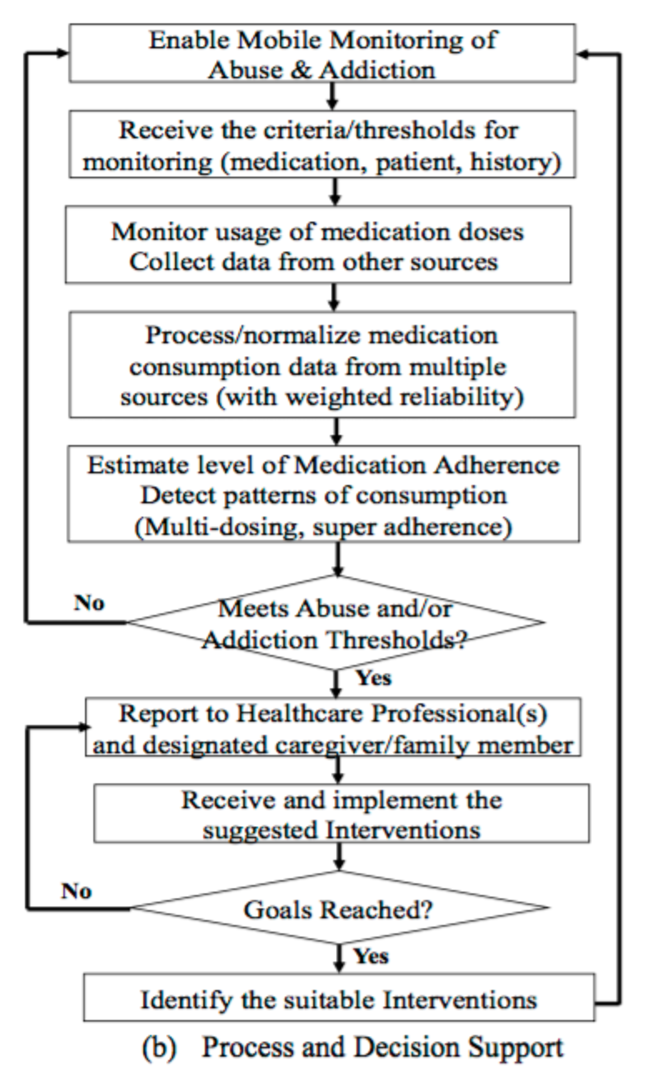
\includegraphics[width=\columnwidth]{images/Figure1.pdf}
  \caption{Drugs Involved in U.S. Overdose Deaths from 2000 to 2016, 
  National Institute on Drug Addiction (NIDS) \cite{nida17}
  }\label{f:Figure1}
\end{figure}

%%%%%%%%%%%%%%%%%%%%%%%%%%%%%%%%%%%%%%%%%%%%%%%%%%%%%%%%%%%%%%%%%%%%%%%%%%%%%%%%%%
\subsubsection{Drug Addiction and Treatment}

For millions of people struggling with substance abuse and dependency in 
the U.S., addiction and relapse are chronic health conditions \cite{boyer10}. 
Drug addiction has many similar characteristics to other chronic medical 
illnesses; however, there are unique challenges to the treatment of addiction
illnesses. For example, drug addicted patients undergo intense detoxification 
in rehabilitation treatment programs, which reduces their drug tolerance, and 
then are released back into the same environment associated with their drug use, 
putting them at greater risk for relapse and potential drug overdose. The lack 
of continuity in the treatment of addiction disorders leaves persons in recovery 
at high risk of relapse for substance use and abuse. Second, individuals with 
severe addiction disorders end up at emergency rooms for care following acute 
intoxication, often following law enforcement interventions. Emergency personal 
are very competent at crisis interventions for drug overdose, but lack resources 
to evaluate severe addiction disorders or provide follow-up. Furthermore, 
addicted individuals seeking treatment often relapse at night or on weekends 
when treatment centers are not open. Various theories of addiction and relapse 
have been proposed. According to the classical conditioning model, situational 
cues or events can elicit a motivational state underlying relapse to drug use. 
A slightly more complex model suggests that addictive behavior can be reinstated 
after extinction of dependency by exposure to drugs, drug-related cues, or 
environmental stressors \cite{shaham03}. Understanding that a user`s affective
(i.e., motivational) response to cues in the environment can lead to relapse 
and drug use are key to developing strategies for prevention and treatment. 

%%%%%%%%%%%%%%%%%%%%%%%%%%%%%%%%%%%%%%%%%%%%%%%%%%%%%%%%%%%%%%%%%%%%%%%%%%%%%%%%%%
\subsection{Technology-Based Interventions for Addiction Treatment}

Technology-based interventions have been used for drug addiction assessment, 
treatment, prevention, and recovery \cite{marsch12}. In terms of assessment, 
data about substance use can be obtained from mobile cell phone reporting 
outside of treatment settings. Web-based approaches to treatment have been 
implemented online to improve behavioral and psychosocial functioning for 
addicted individuals in recovery \cite{marschdallery2012}. For example, the 
{\em Therapeutic Education System} (TES) is a self-directed, web-based 
interactive treatment program consisted of 65 training modules that focused 
on cognitive-behavioral skills and psychosocial functioning (family/social 
relations). This online approach helped to increase access to treatment for 
individuals in rural areas, and included an optional contingency management 
module. A computer based {\em Training in Cognitive Behavioral Therapy} (CBT) 
program was found to enhance treatment outcomes when provided in conjunction 
with traditional substance abuse treatment, and helped improve coping skills 
and decision-making skills \cite{carroll08}. In evaluating the effectiveness 
of mobile applications for addiction treatment, several questions remain to be 
answered: First, if mobile applications are regarded primarily as supplements 
to traditional therapeutic treatment, can their effectiveness be evaluated 
independently from the approach used in treatment? Second, over what time 
period period can the benefits of mobile applications be observed? Research 
evidence suggests that the benefits of mobile interventions may be limited 
to 12 or 15 weeks \cite{swedenson16}. It is unclear whether individuals 
struggling from addiction would continue to use mobile treatment applications 
in the long term, beyond a limited course of treatment.


%%%%%%%%%%%%%%%%%%%%%%%%%%%%%%%%%%%%%%%%%%%%%%%%%%%%%%%%%%%%%%%%%%%%%%%%%%%%%%%%%%
\subsubsection{Mobile-Based Applications}

Mobile applications have been used for monitoring and treatment of substance 
abuse and addiction disorders for several decades \cite{boyer10}. Early 
applications included the use of electronic pagers (i.e., beepers) for 
experience sampling with paper-based assessments that generated data about 
daily life behavior and experiences \cite{swedenson16}. In the 1990s, 
programmable personal digital assistants (e.g., palm-pilot) enabled collection 
of data electronically, and subsequent mobile research tools facilitated the 
collection of information about psychological factors (e.g., daily stressors, 
emotional states, thoughts) and other variables related to addiction (e.g., 
craving, contextual cues, actual substance use). Assessments performed several 
times throughout the day (commonly, every 2 to 4 hours) allowed for analysis of 
the daily fluctuations of these symptoms and features. Historically, addiction 
research has faced some unique challenges that the use of mobile technologies 
may help to overcome. Methodological aspects of traditional research using 
retrospective, cross-sectional, or longitudinal assessments (over periods of 
weeks, months, or years) have been problematic for investigating risk factors 
including behaviors and symptoms (severe physiological cravings, withdrawal, 
and substance use) that can span a relatively short time. An additional factor 
is the co-morbidity, or co-occurence, of substance use disorders (SUDs) with 
other psychological disorders, such as anxiety and mood disorders. For example, 
the {\em self-medication} model has commonly been used to explain the association 
between alcohol abuse as an effort by an individual to reduce or cope with a 
high degree of anxiety (or depression). It has also been challenging for 
researchers to capture the role of environmental or contextual cues (e.g., 
people, places, things) associated with substance abuse, which can act as 
triggers of relapse for individuals in recovery.


%%%%%%%%%%%%%%%%%%%%%%%%%%%%%%%%%%%%%%%%%%%%%%%%%%%%%%%%%%%%%%%%%%%%%%%%%%%%%%%%%%
\subsubsection*{Smartphone Applications}

Continued care is an important ingredient for recovery from addiction that
involves monitoring, outreach, planning, case management, and social support 
\cite{johnson11}. Smartphone applications can help individuals in recovery to 
monitor cravings at critical points in daily life, track contextual cues 
associated with substance use, and provide outreach to support services. A team 
of researchers at the University of Wisconsin evaluated the effectiveness of a
smartphone application called {\em Addiction Comprehensive Health Enhancement 
Support System} (A-CHESS), designed to provide recovery support for patients 
leaving a residential alcohol treatment center \cite{gustafson14}. A-CHESS 
provided anytime, anywhere access to support services in audio-visual format, 
GPS monitoring and warnings for risky locations related to past substance use, 
and communication with counselors. Over an 8-month period (and 4 month follow-up), 
patients who used the A-CHESS intervention reported fewer risky drinking days, 
on average, per month than patients in a comparable control group. The findings 
provide evidence that the smartphone intervention was effective at treating a 
critical behavioral measure for treatment of alcohol use disorder (AUD). The 
methods described in this study could be extended by re-purposing built-in 
smartphone sensors to record physiological measures related to opioid usage, 
and communicate data to health care providers or treatment specialists to 
initiate interventions for opioid addiction \cite{johnson11}. 

\begin{figure}[!ht]
  \centering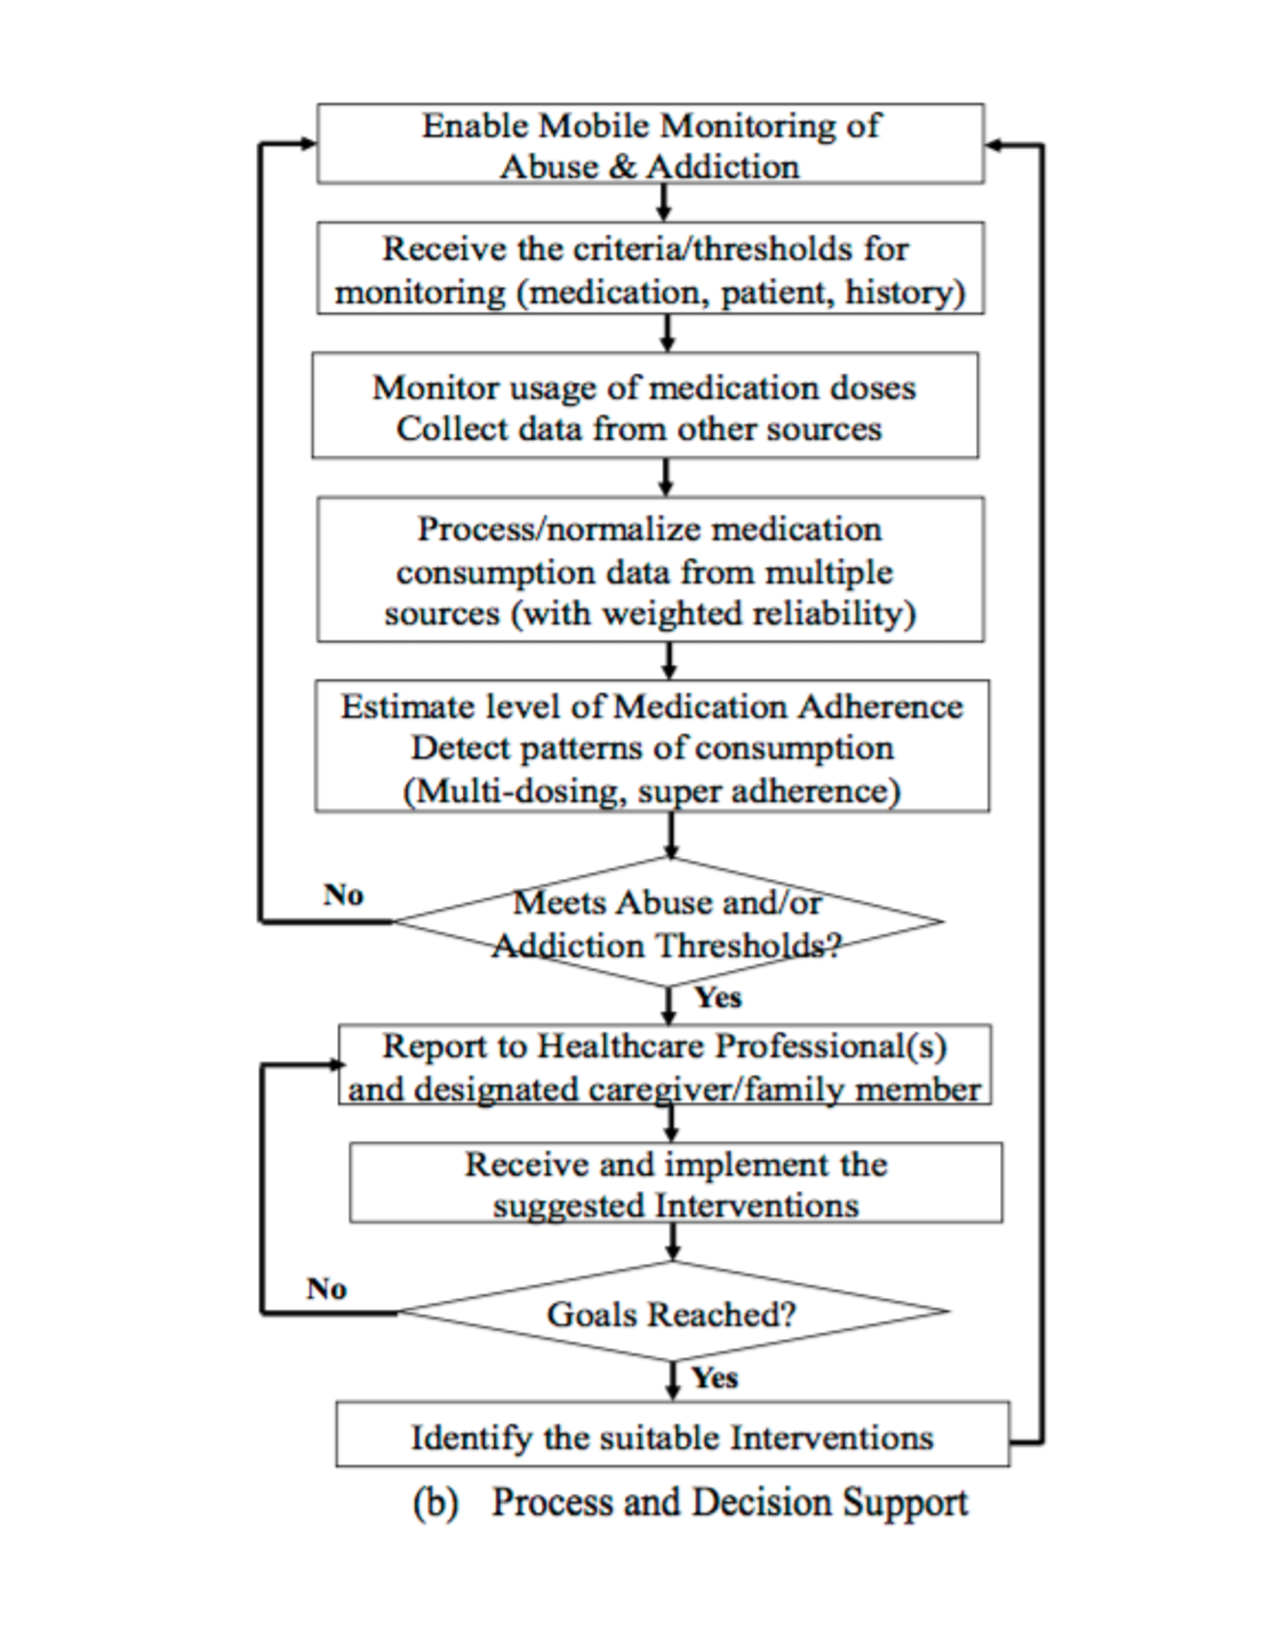
\includegraphics[width=\columnwidth]{images/Figure2.pdf}
  \caption{Process and Decision Support for Abuse Monitoring System 
  \cite{Varshney14}
  }\label{f:Figure2}
\end{figure}

%%%%%%%%%%%%%%%%%%%%%%%%%%%%%%%%%%%%%%%%%%%%%%%%%%%%%%%%%%%%%%%%%%%%%%%%%%%%%%%%%%
\subsection{Medication Adherence and Abuse Monitoring System}

Mobile health applications can be used to monitor medication adherence and 
as an advanced warning system for potential abuse of prescription medication 
\cite{varshney13}. Medication abuse can consist of higher medication dosages 
or rapid escalation of a prescribed dosage, and the general goal of a prediction 
model is to analyze patient data for sudden changes in medication consumption. 
Figure 2 illustrates several steps in a process and decision support structure 
for a medication monitoring system, with adjustable parameters, such as the 
threshold for abuse (e.g., greater than N doses in X hours) \cite{Varshney14}. 
A major challenge for measuring medication abuse is obtaining reliable 
information from potentially addicted individuals based on self report data. 
Ideally, information on medication consumption and adherence can be obtained 
from multiple sources. Addiction is a complex behavior that involves a variety 
of factors, including: demographics (e.g., age, gender), past history, 
comorbidity with other disorders, family support, social influence, employment 
status, and patient motivation. Figure 3 shows a model architecture of a system 
for monitoring potential abuse where dose information is provided via a 
smartphone application, relayed via wireless cellular network to analytic models 
that measure changes in medication consumption, relays reports to support 
treatment services for possible interventions, and to a smart medication box that 
dispenses medication. In order to function successfully a medication abuse 
monitoring system depends on the collection of reliable information, including 
data from wearable sensors that can directly measure physiological changes 
(e.g., heartrate, blood pressure, respiration, temperature) related to changes 
in medication usage. In the context of prescription opioid abuse, a medication 
monitoring system could be very beneficial in anticipating opioid dependency
and preventing accidental death from medication overdose. 

\begin{figure}[!ht]
  \centering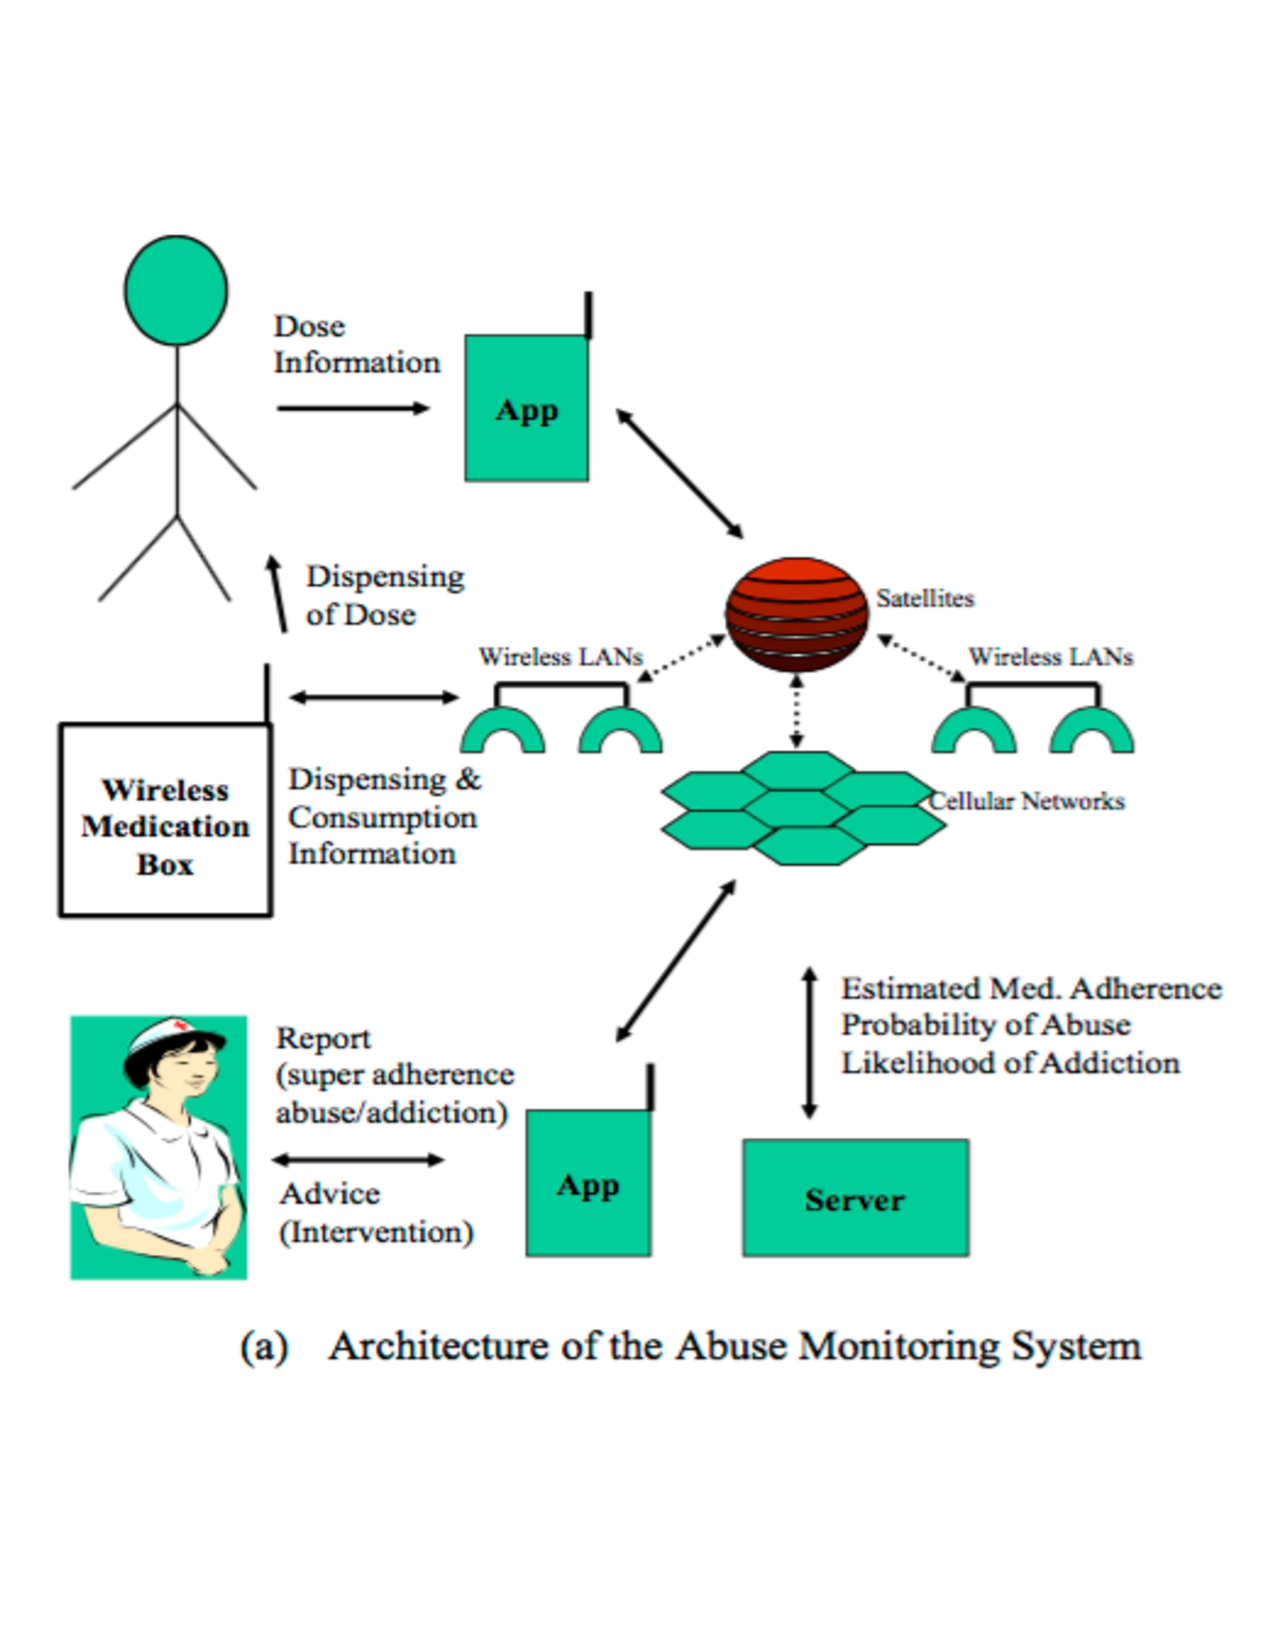
\includegraphics[width=\columnwidth]{images/Figure3.pdf}
  \caption{Architecture for Abuse Monitoring System \cite{Varshney14}
  }\label{f:Figure3}
\end{figure}

%%%%%%%%%%%%%%%%%%%%%%%%%%%%%%%%%%%%%%%%%%%%%%%%%%%%%%%%%%%%%%%%%%%%%%%%%%%%%%%%%%
\subsection{Mobile Detection with Wearable Biosensors}

Portable biosensors can provide a continuous stream of data on the timing, 
location, context, and duration of drug use by individuals in treatment. 
In a small pilot study, researchers used an Affectiva Q sensor to measure 
electrodermal activity (EDA), skin temperature, and acceleration (8 recordings 
per second), in a sample of N = 4 patients during the administration of opioid 
medication in an emergency room setting \cite{carreiro15}. Table 1 provides a 
summary of the participant characteristics. The biosensor was worn on the 
wrist and was similar in size and dimensions to a wristwatch or fitbit health
monitor. The results showed an increase in EDA associated with intravenous 
opioid injection that was detected by the biosensors. In addition, there was 
some indication that the physiological response to opioids varied according 
to individual drug tolerance; patients with higher opioid tolerance showed
less EDA response than patients with low tolerance. The findings provide 
evidence to support the use of wearable sensors to detect drug use in real 
time, in a controlled environment. An important limitation of the study is 
the small sample size, which reduces the generalizability of the findings to 
a broader population. The authors also acknowledged that psychological or 
physiological stress can produce alterations in EDA, skin temperature, and 
acceleration, and therefore this could not be ruled out as an alternative 
explanation for the findings. The results are promising, however, and 
encourage efforts to explore the effectiveness of wearable biosensors 
in the context of environments associated with substance use.

\begin{table}
  \caption{Summary of Participant Characteristics in Pilot study \cite{carreiro15}}
  \label{tab:freq}
  \begin{tabular}{ccccccc}
    \toprule
     Patient& Age& Gender& History of Use& Intervention& Pre-EDA& Post-EDA \\
    \midrule
    1& 82& Male& Opioid naive& 4 mg morphine& 4.5& 60.0 \\
    2& 47& Male& Recent short-term& 1 mg hydromorphone& 3.4& 12.2 \\
    3& 43& Female& Chronic opioid use& 1 mg hydromorphone& 0.2& 0.2 \\
    4& 72& Male& Chronic opioid use& 4 mg morphine& 0.9& 1.6 \\
    \bottomrule
  \end{tabular}
\end{table}

%%%%%%%%%%%%%%%%%%%%%%%%%%%%%%%%%%%%%%%%%%%%%%%%%%%%%%%%%%%%%%%%%%%%%%%%%%%%%%%%%%
\subsection{Emerging Sensor Technologies}

Wearable wireless sensors have been used to study physiological responses, 
activity, and social behavior in non-human primates in the form of a fitted 
vest and using a mobile phone with blue tooth protocol to collect data 
in real time. Figure 4 shows sample ambulatory data from a rhesus macaque
recorded from a wearable wireless sensor for 11 hours inside a large group 
primate cage \cite{fletcher12}. Data was recorded on a custom Android software 
application, which captured measures of EDA, heart rate (HR), temperature, and 
acceleration. The goals of this study were to measure associations between 
physiological measures and social behavior in primates; however, this practical 
application of sensor technology demonstrated a system that was relatively 
low-cost, highly portable, scalable, and simple to use. Future research could 
explore the development of a similar system modified for use with humans to 
collect data on physiological measures from addicted individuals in naturalistic 
settings. 

\begin{figure}[!ht]
  \centering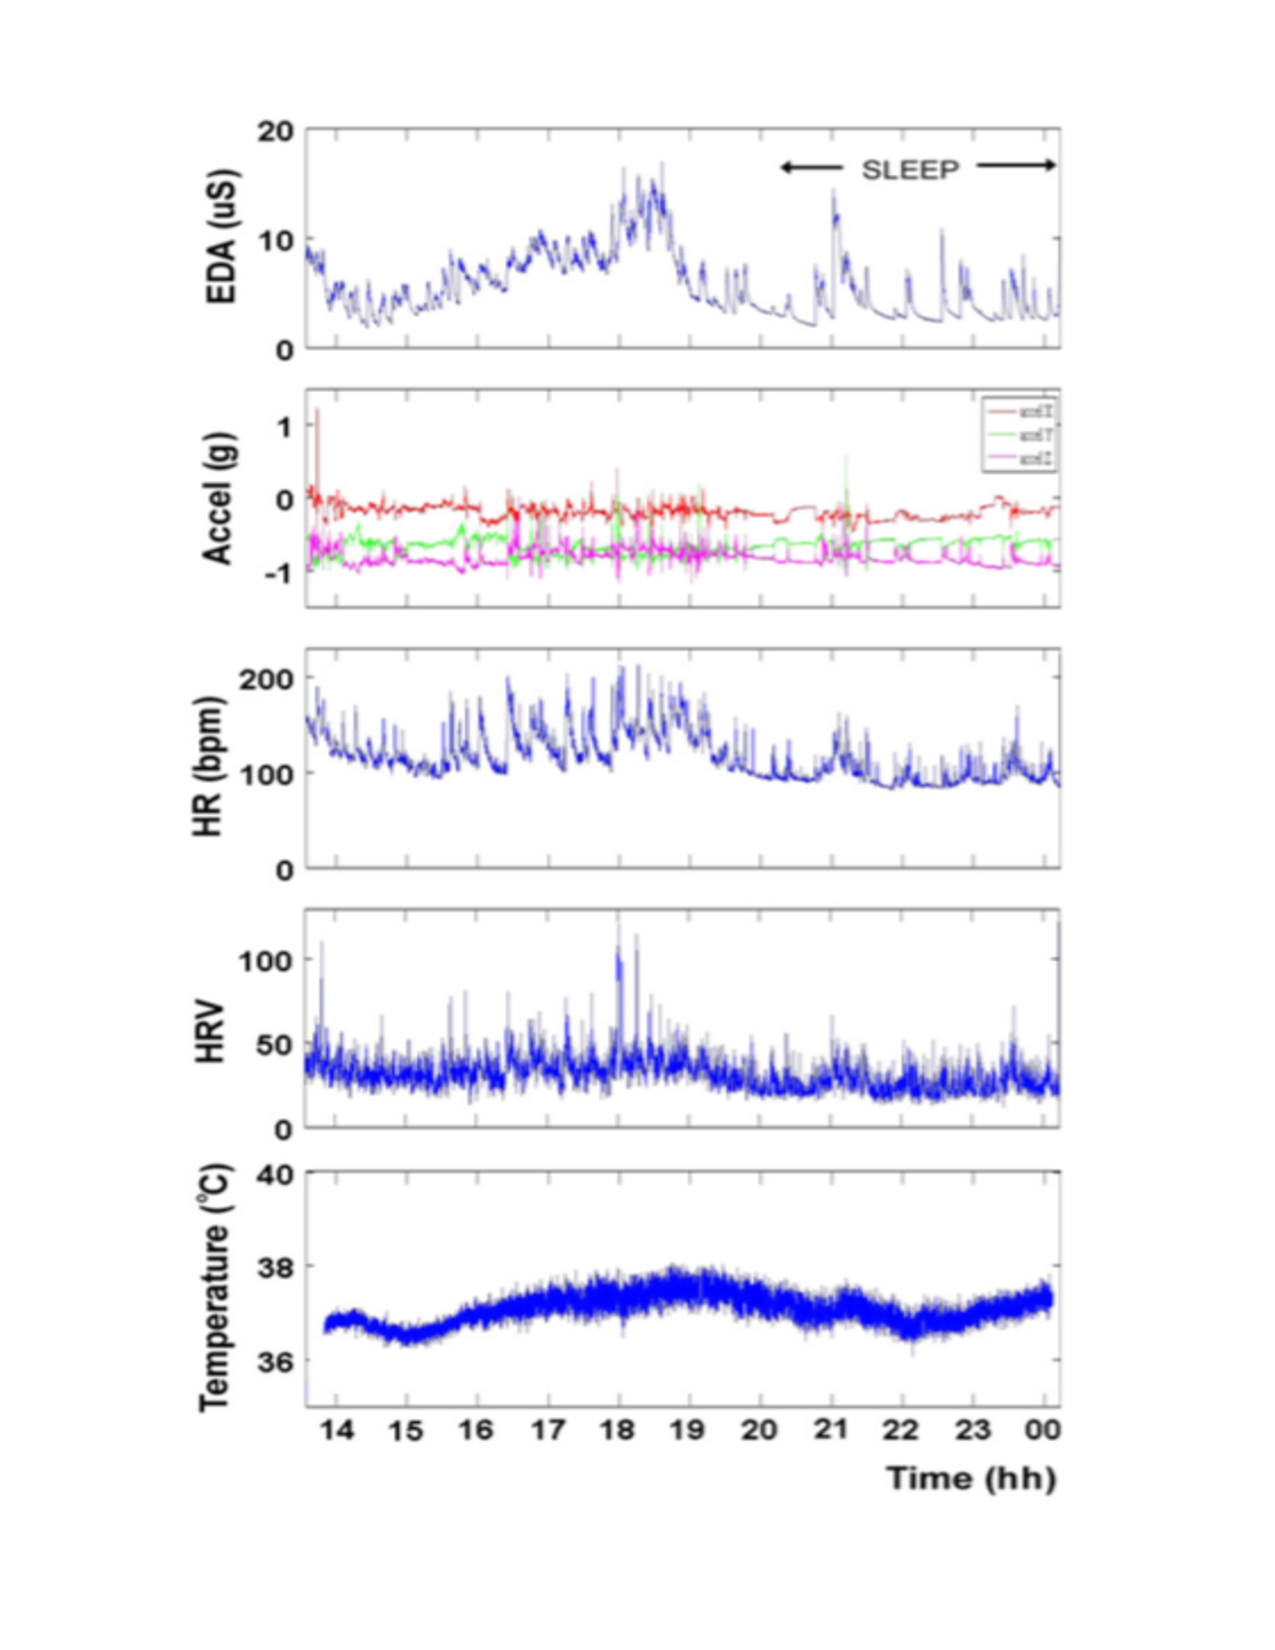
\includegraphics[width=\columnwidth]{images/Figure4.pdf}
  \caption{Sample Ambulatory Data from Rhesus Macaque Recorded on 
  Wearable Sensor for 11+ hours Inside Large Primate Cage Facility 
  \cite{fletcher12}}
  \label{f:Figure4}
\end{figure}

%%%%%%%%%%%%%%%%%%%%%%%%%%%%%%%%%%%%%%%%%%%%%%%%%%%%%%%%%%%%%%%%%%%%%%%%%%%%%%%%%%
\subsubsection{LoRa Backscatter: Enabling Ubiquitous Connectivity} 

Emerging technologies, such as longe range (LoRa) backscatter, have the potential 
to extend the boundaries of wireless connectivity. Existing radio technologies 
(e.g., WIFI, ZigBee, SigFox, LTE-M) provide reliable long range coverage, but 
consume energy and would be costly to expand to large scale implementation; 
however, LoRa backscatter is a smaller, low-cost, low-power alternative with 
extended range between an RF source and receiver of approximately 475 meters 
(i.e., yards) \cite{talla17}. Table 1 shows the sensitivity and supported data 
rates for different communication technologies and  feasibility of different 
power sources. LoRa backscatter performed best overall, in terms of sensitivity 
(-149 dBm), supporting bit rates of 18 pbs to 37.5 kbps, providing whole home 
coverage, and capable of being powered by button cell, tiny solar cell, or 
printed battery. LoRa backscatter uses chirp spread activation (CSS) that can 
synthesize continuous frequency modulated chirps; a limitation is that 
backscatter is drowned out by noise and the RF source. The LoRa backscatter 
system was tested in various deployments: across three floors of a 4800 square-
foot house, a single floor of 13,000 square foot office building, and on a 
one-acre farm. Figure 5 shows the layout of the house with the RF source (TX) 
on the second floor and receiver in the basement (RX); the plot shows the system 
achieved RSSI values greater than -144 dBm, with reliable wireless coverage 
throughout the house, and rates sufficient for temperature sensors that 
transmit small packages. The system was also implemented in the form flexible 
epidermal patch sensor shown in Figure 6, that provided reliable connectivity 
across a 3,300 square foot atrium with RSSI greater than -132 dBm. LoRa 
backscatter provides a compact, energy-efficient, and affordable wireless 
transmission system that can be extended to scale at reasonable cost. This 
system could possibly transmission of biometric data from wearable sensors 
to capture health information from addicted individuals in treatment. 

\begin{table}
  \caption{Comparison of Wireless Communication Technologies \cite{talla17}}
  \label{tab:freq}
  \begin{tabular}{ccccccc}
    \toprule
     Technology& Sensitivity& Data Rate& Home Coverage& Button Cell& Tiny Solar Cell& Printed Battery \\
    \midrule
    Wi-Fi (802.11 b/g)& -95 dBm& 1-54 Mbps& yes& no& no& no \\
    LoRa& -149 dBm& 18 bps-37.5 kbps& yes& no& no& no \\
    Bluetooth& -97 dBm& 1-2 Mbps& no& no& no& no \\
    SigFox& -126 dBm& 100 bps& yes& no& no& no \\
    Zigbee& -100 dBm& 250 kpbs& yes& no& no& no \\
    Passive Wi-Fi& -95 dBm& 1-11 Mbps& no& yes& yes& yes \\
    RFID& -85 dBm& 40-640 kbps& no& yes& yes& yes \\
    LoRA Backscatter& -149 dBm& 18 bps-37.5 kpbs& yes& yes& yes& yes \\
    \bottomrule
  \end{tabular}
\end{table}

\begin{figure}[!ht]
  \centering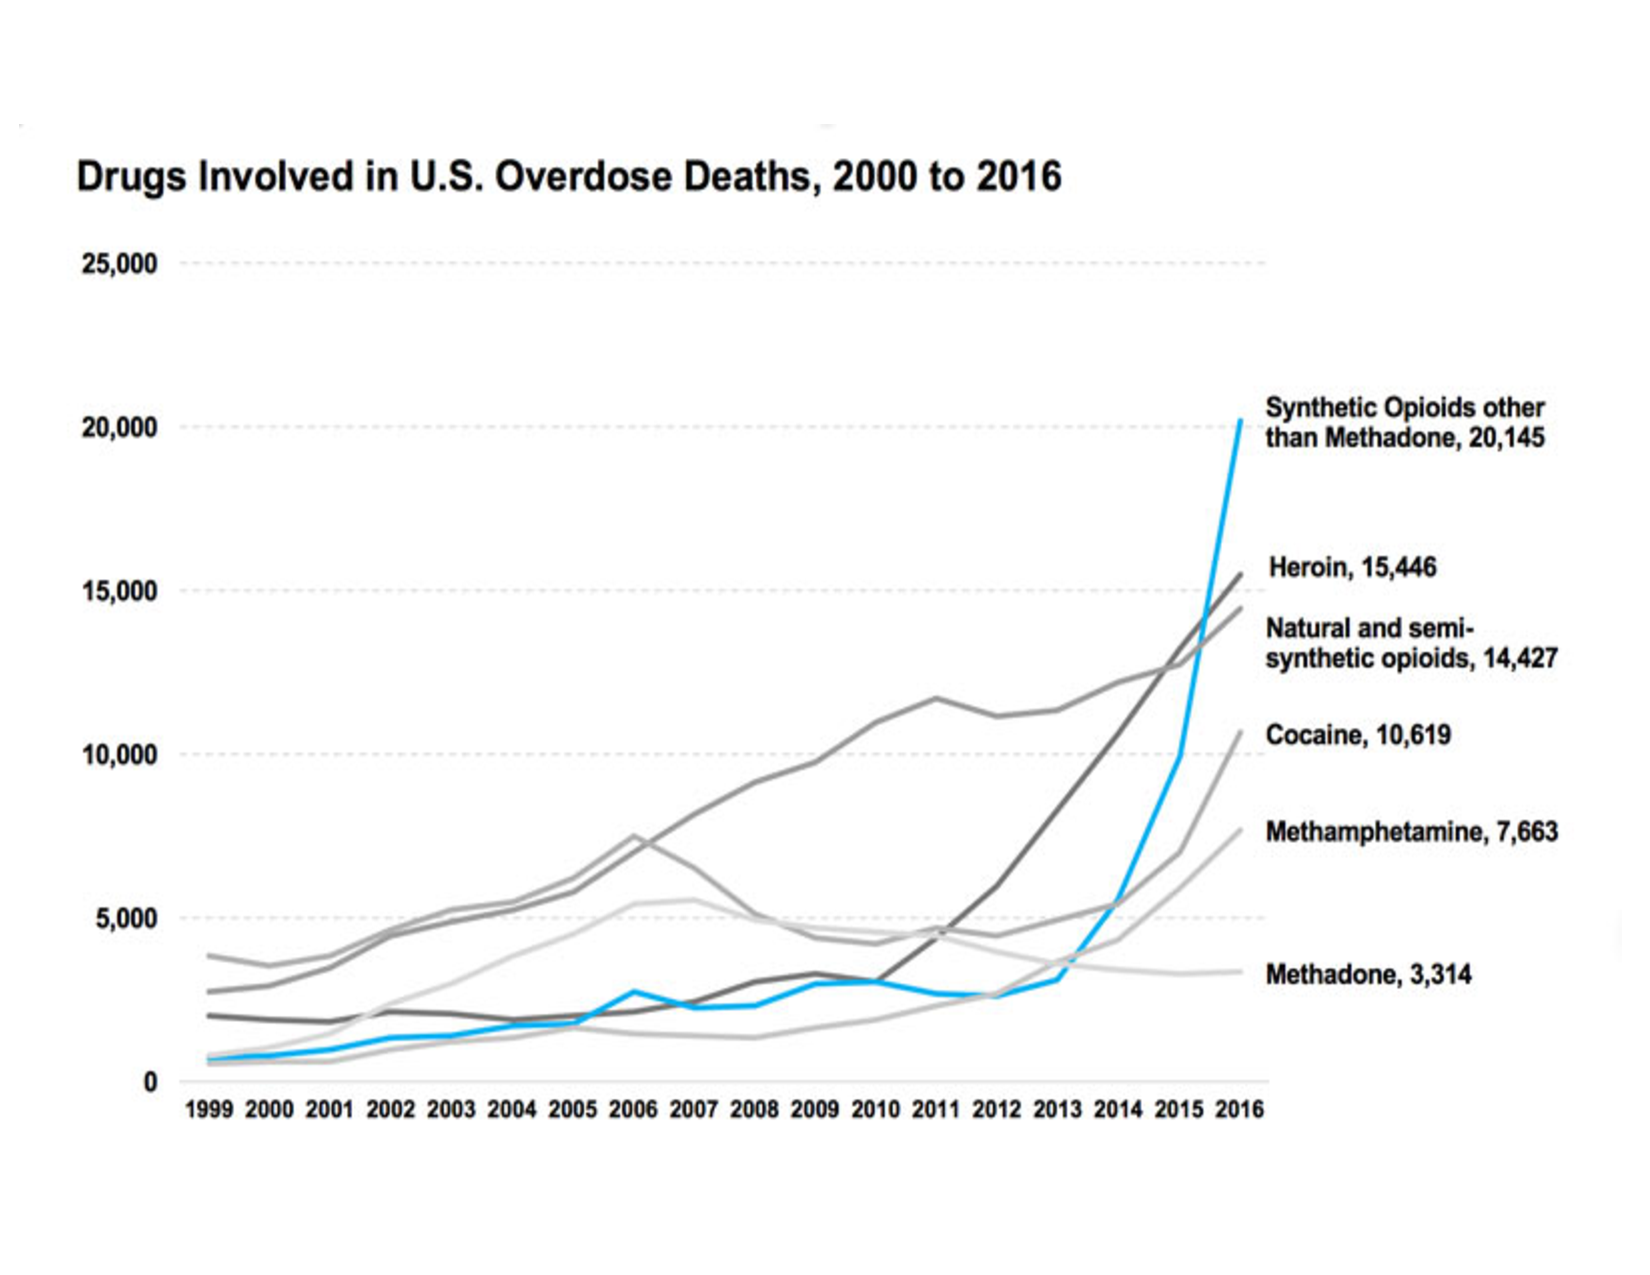
\includegraphics[width=\columnwidth]{images/Figure5.pdf}
  \caption{Home Deployment of LoRa backscatter pakcets across 4,800 sq. ft.
  House Apread Across Three Floors \cite{talla17}
  }\label{f:Figure5}
\end{figure}

\begin{figure}[!ht]
  \centering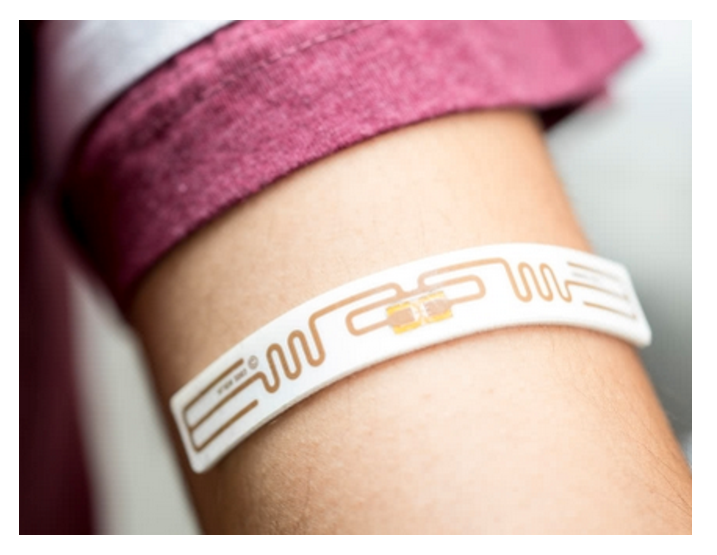
\includegraphics[width=\columnwidth]{images/Figure6.pdf}
  \caption{LoRa Backscatter Epidermal Patch \cite{talla17}
  }\label{f:Figure6}
\end{figure}

%%%%%%%%%%%%%%%%%%%%%%%%%%%%%%%%%%%%%%%%%%%%%%%%%%%%%%%%%%%%%%%%%%%%%%%%%%%%%%%%%%
\subsubsection{Graphene Electronic Tattoo sensors}

Wearable, tattoo-like epidermal sensors allow for continuous, ambulatory 
monitoring of biometric signals from the heart, muscles, and brain, outside of
hospitals and clinical lab settings \cite{bourzac17}. A team of researchers at 
the University of Texas at Austin designed the graphene electronic tattoo (GET)
as a long term wearable sensor that can be directly laminated on human skin, 
and can remain functional for several days with a liquid bandage cover 
\cite{ameri17}. Graphene is the thinnest electrically conductive material
that is biocompatible, stable, and mechanically robust. The ``GET is 
fabricated through a simple `wet transfer, dry patterning` process directly
on tattoo paper, allowing it to be transferred  on human skin exactly like 
a temporary tattoo, except the sensor is transparent``(p.8)\cite{ameri17}. 
As depicted in Figure 7, the GET sensor is is flexible, stretchable, and 
transparent, and less than a sub-micrometer in thickness (463 +/- 30 nm). 
GET has been used successfully to measure electrocardiograph (ECK), 
electromyogram (EMG), electrocephalograph (EEG) signals, as well as skin 
temperature and skin hydration. After use, the GET can be easily removed by 
peeling it from the skin. A future step in the development of GET is to include
an antenna to the design so that signals can be beamed off the device to a
smartphone application or computer. The thin, flexible, resilient tattoo 
biosensor provides a durable, unobtrusive tool for collecting physiological 
data, and could be used to detect physical changes due to drug withdrawal 
in addicted individuals. 

\begin{figure}[!ht]
  \centering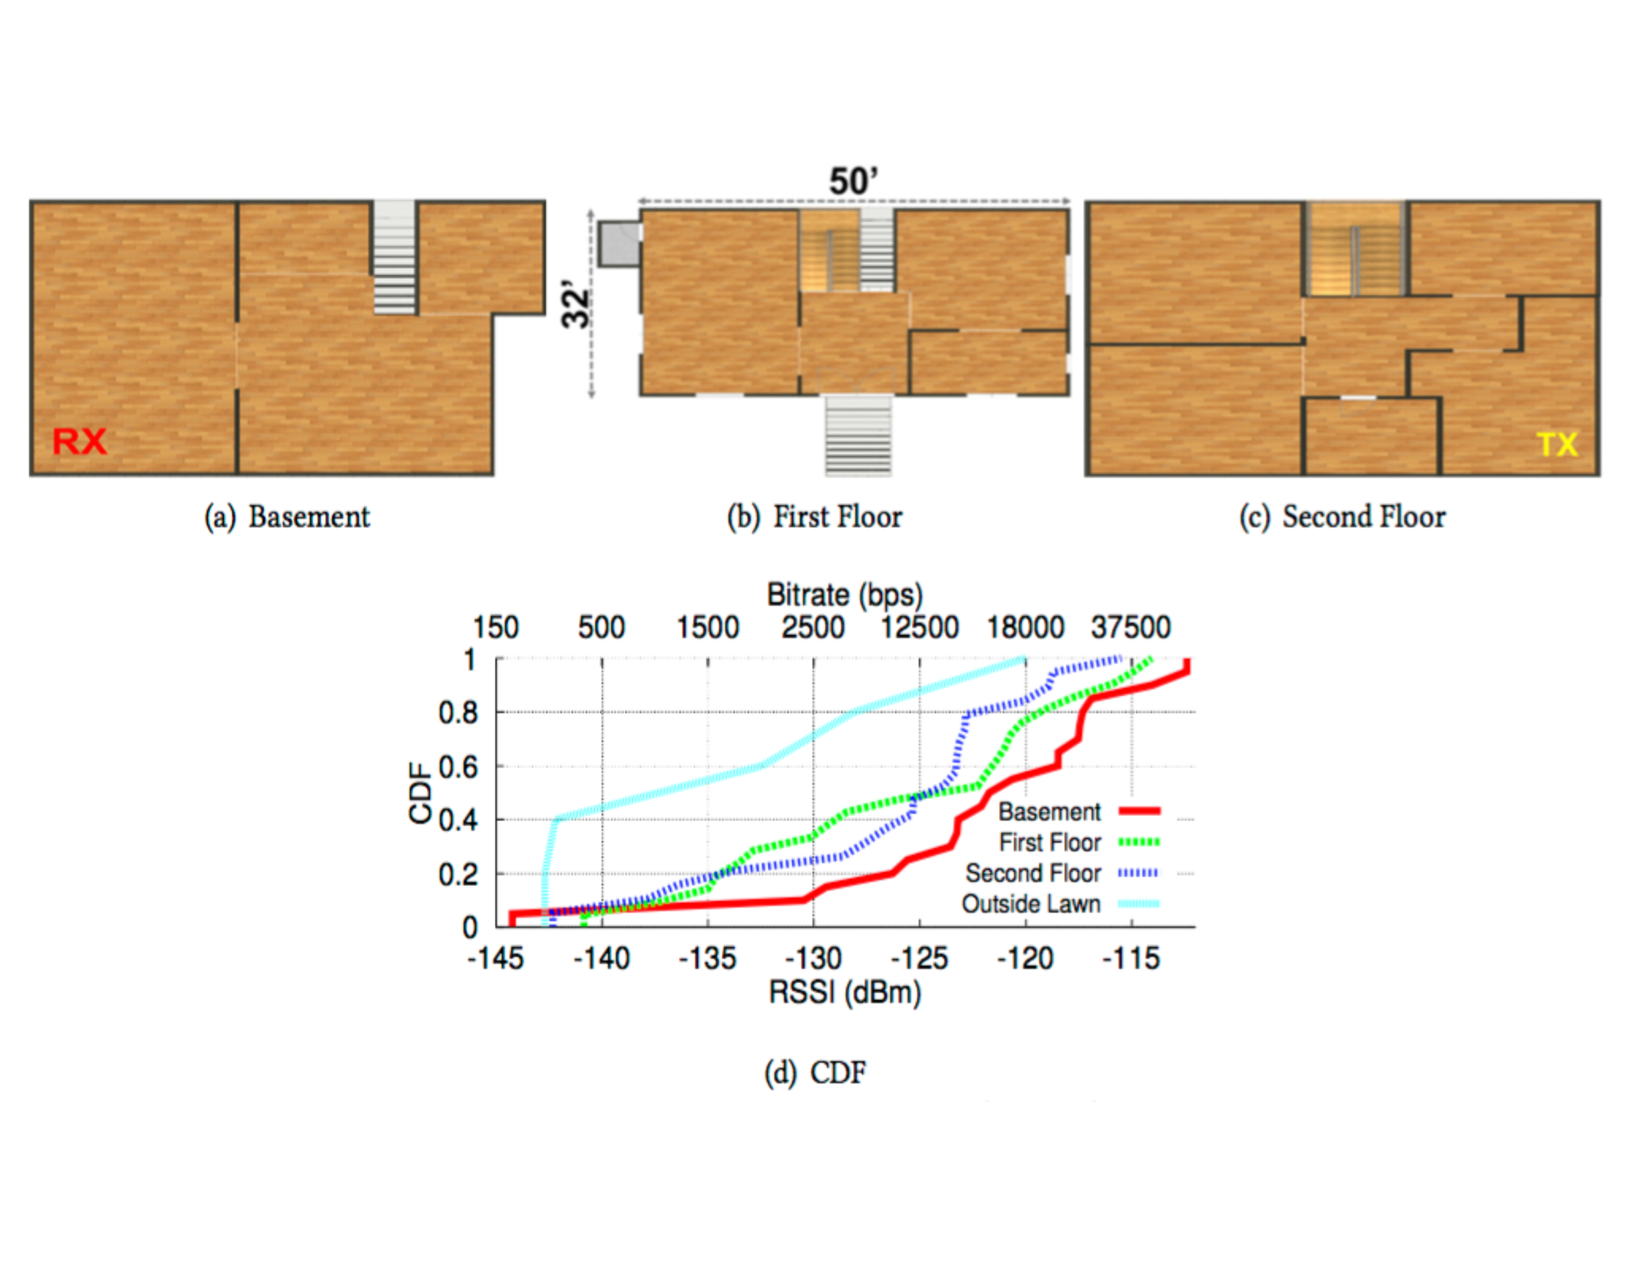
\includegraphics[width=\columnwidth]{images/Figure7.pdf}
  \caption{Graphene Electronic Tatoo Biosensor \cite{ameri17}
  }\label{f:Figure7}
\end{figure}

%%%%%%%%%%%%%%%%%%%%%%%%%%%%%%%%%%%%%%%%%%%%%%%%%%%%%%%%%%%%%%%%%%%%%%%%%%%%%%%%%%

\section{Conclusion}

{\em Can Technological Applications Reduce Opioid Addiction?}
The abuse of prescription medication in the U.S. has led to opioid addiction  
at levels of epidemic proportion. Technological interventions can play a role 
in addressing this crisis as a supplement to conventional forms of addiction 
treatment. Mobile health applications can help monitor potential medication 
abuse and connect individuals with treatment services. An important limitation 
of data based addiction interventions is the difficulty of obtaining reliable 
information about medication consumption based on self-reports from potentially 
addicted individuals. The literature reviewed indicates that wearable sensors 
are an effective way to measure vital health data in real time and remotely. 
Providing individuals in recovery with vital health data may help them to 
resist physical cravings and prevent relapse. Another limitation of treatment 
approaches is that, after detoxification, individuals in recovery are released 
back into the environmental settings associated with their drug use, putting 
them at risk for potential relapse and possible overdose. Recent advances in 
signal technologies such as LoRa Backscatter and Graphene tattoo sensors can 
lead to the more efficient collection of biometric information and cost 
effective transmission of health data for subsequent analysis. The opioid 
addiction epidemic is a complex phenomenon, with both physical and sociological 
contributing factors. Technological interventions will increase the amount of 
data about addicted individuals and relevant risk factors that may be used to 
predict opioid overdose death; however, it will not address the environmental
factors that lead to addiction. Despite increased awareness of the potential 
for prescription medication abuse, Table 1 shows the rate of overdose deaths 
is growing more rapidly for heroin and synthetic opioids such as fentanyl 
compared to conventional prescription opioid medication. The implication of 
this is that individuals who may become addicted to prescribed medication may 
go on to abuse illicit or synthetic opioids, in non-clinical, unsupervised,
and unregulated settings. Big data offers potential for transforming health 
care and addition treatment. Increasing levels of data about opioid 
addiction ultimately may not be sufficient to prevent or decrease rates of 
overdose death if the availability of illicit and synthetic opioids remains 
high. 


%%%%%%%%%%%%%%%%%%%%%%%%%%%%%%%%%%%%%%%%%%%%%%%%%%%%%%%%%%%%%%%%%%%%%%%%%%%%%%%%%%

\begin{acks}

    The author would like to thank Dr. Gregor von Laszewski, 
    the Assistant Instructors, Juliette Zurick and others, and 
    anonymous reviewers who helped to improve this report. 

\end{acks}

\bibliographystyle{ACM-Reference-Format}
\bibliography{report} 

\section{Issues}

\DONE{Example of done item: Once you fix an item, change TODO to DONE}

\subsection{Assignment Submission Issues}

    \DONE{Do not make changes to your paper during grading, when your repository should be frozen.}

\subsection{Uncaught Bibliography Errors}

    \DONE{Missing bibliography file generated by JabRef}
    \DONE{Bibtex labels cannot have any spaces, \_ or \& in it}
    \DONE{Citations in text showing as [?]: this means either your report.bib is not up-to-date or there is a spelling error in the label of the item you want to cite, either in report.bib or in report.tex}

\subsection{Formatting}

    \DONE{Incorrect number of keywords or HID and i523 not included in the keywords}
    \DONE{Other formatting issues}

\subsection{Writing Errors}

    \DONE{Errors in title, e.g. capitalization}
    \DONE{Spelling errors}
    \DONE{Are you using {\em a} and {\em the} properly?}
    \DONE{Do not use phrases such as {\em shown in the Figure below}. Instead, use {\em as shown in Figure 3}, when referring to the 3rd figure}
    \DONE{Do not use the word {\em I} instead use {\em we} even if you are the sole author}
    \DONE{Do not use the phrase {\em In this paper/report we show} instead use {\em We show}. It is not important if this is a paper or a report and does not need to be mentioned}
    \DONE{If you want to say {\em and} do not use {\em \&} but use the word {\em and}}
    \DONE{Use a space after . , : }
    \DONE{When using a section command, the section title is not written in all-caps as format does this for you}\begin{verbatim}\section{Introduction} and NOT \section{INTRODUCTION} \end{verbatim}

\subsection{Citation Issues and Plagiarism}

    \DONE{It is your responsibility to make sure no plagiarism occurs. The instructions and resources were given in the class}
    \DONE{Claims made without citations provided}
    \DONE{Need to paraphrase long quotations (whole sentences or longer)}
    \DONE{Need to quote directly cited material}

\subsection{Character Errors}

    \DONE{Erroneous use of quotation marks, i.e. use ``quotes'' , instead of " "}
    \DONE{To emphasize a word, use {\em emphasize} and not ``quote''}
    \DONE{When using the characters \& \# \% \_  put a backslash before them so that they show up correctly}
    \DONE{Pasting and copying from the Web often results in non-ASCII characters to be used in your text, please remove them and replace accordingly. This is the case for quotes, dashes and all the other special characters.}
    \DONE{If you see a figure and not a figure in text you copied from a text that has the fi combined as a single character}

\subsection{Structural Issues}

    \DONE{Acknowledgement section missing}
    \DONE{Incorrect README file}
    \DONE{In case of a class and if you do a multi-author paper, you need to add an appendix describing who did what in the paper}
    \DONE{The paper has less than 2 pages of text, i.e. excluding images, tables and figures}
    \DONE{The paper has more than 6 pages of text, i.e. excluding images, tables and figures}
    \DONE{Do not artificially inflate your paper if you are below the page limit}

\subsection{Details about the Figures and Tables}

    \DONE{Capitalization errors in referring to captions, e.g. Figure 1, Table 2}
    \DONE{Do use {\em label} and {\em ref} to automatically create figure numbers}
    \DONE{Wrong placement of figure caption. They should be on the bottom of the figure}
    \DONE{Wrong placement of table caption. They should be on the top of the table}
    \DONE{Images submitted incorrectly. They should be in native format, e.g. .graffle, .pptx, .png, .jpg}
    \DONE{Do not submit eps images. Instead, convert them to PDF}

    \DONE{The image files must be in a single directory named "images"}
    \DONE{In case there is a powerpoint in the submission, the image must be exported as PDF}
    \DONE{Make the figures large enough so we can read the details. If needed make the figure over two columns}
    \DONE{Do not worry about the figure placement if they are at a different location than you think. Figures are allowed to float. For this class, you should place all figures at the end of the report.}
    \DONE{In case you copied a figure from another paper you need to ask for copyright permission. In case of a class paper, you must include a reference to the original in the caption}
    \DONE{Remove any figure that is not referred to explicitly in the text (As shown in Figure ..)}
    \DONE{Do not use textwidth as a parameter for includegraphics}
    \DONE{Figures should be reasonably sized and often you just need to
  add columnwidth} e.g. \begin{verbatim}/includegraphics[width=\columnwidth]{images/myimage.pdf}\end{verbatim}

re


\end{document}
